\section{Particle rendering}

\begin{figure}[ht!]
    \centering
        \subfloat{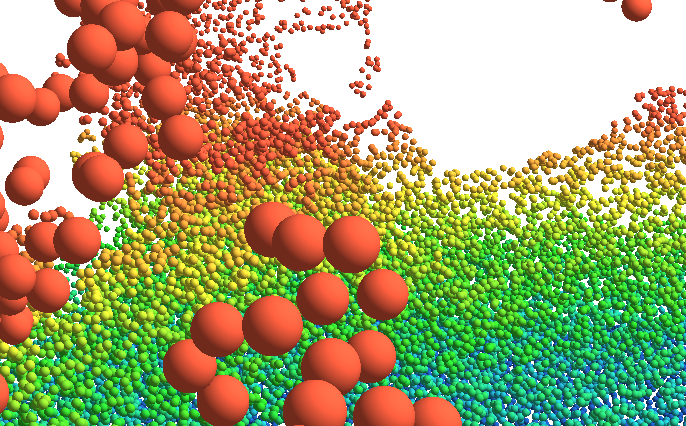
\includegraphics[width=.5\linewidth]{images/part_closeup.png}}
    \caption{Closeup of the shaded particles.}\label{fig:particleShading}
\end{figure}

\noindent
The first step of our pipeline directly draws the particle VBO using \texttt{glDrawArrays()}, which renders each particle as a point sprite. Next, in the vertex shader, we compute the view and projection transforms and set the \texttt{gl\_PointSize} attribute to be proportional to the distance from the projection plane, ensuring that particles further away from the camera appear smaller.\\
The point sprites drawn on screen are squared, and in order to draw a circle, we need to discard those fragments whose distance from the center is greater than one.\\
To shade them as if they were spheres, we can use a simple trick to compute their normal:
\begin{align}
    p &= \texttt{gl\_PointCoord}\nonumber \\
    N &= \begin{pmatrix} p^{\{x\}} & p^{\{y\}} & 1-\|p\|_2\end{pmatrix}\label{eq:sphereEq}
\end{align}

\noindent
Then with the normal, we can use various shading techniques to have a material-light interaction that gives the illusion of having a sphere in the simulation, as shown in Fig. \ref{fig:particleShading}. In our case, we used the Lambertian diffusion lighting model with the Phong ambient component (without the specular highlights); the final color is given by the equation:
\begin{align}
    \texttt{FragColor} = C_{particle} \odot (\alpha \cdot(N\cdot L)) 
\end{align}


\noindent
Where $a$ is the ambient component, $N$ the sphere normal, and $L$ the direction of incident light.\\

\begin{figure}[ht!]
    \centering
        \subfloat[Particle velocity]{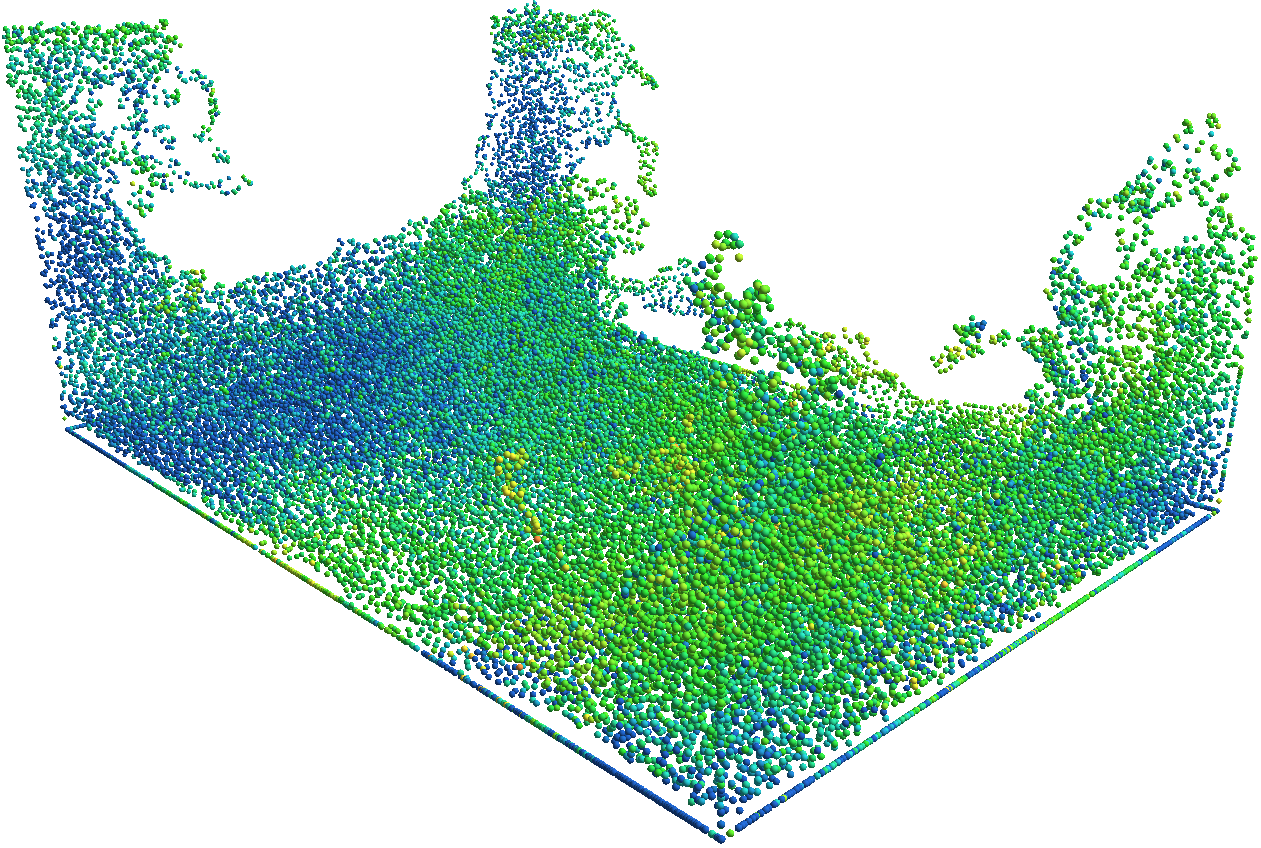
\includegraphics[width=.45\linewidth]{images/part_speed_shader.png}}\hfill
        \subfloat[Particle height]{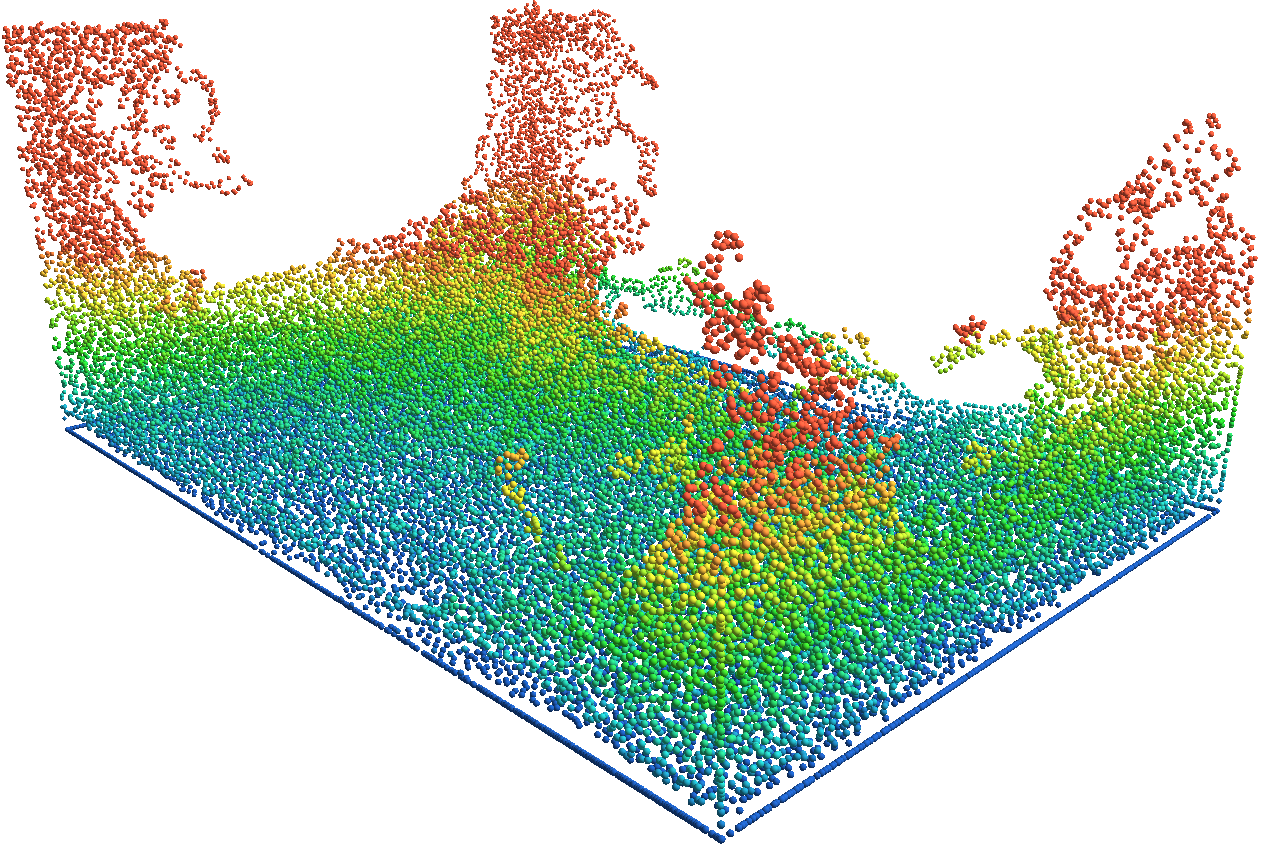
\includegraphics[width=.45\linewidth]{images/part_height_shader.png}}\hfill
        \centering\subfloat[Particle density]{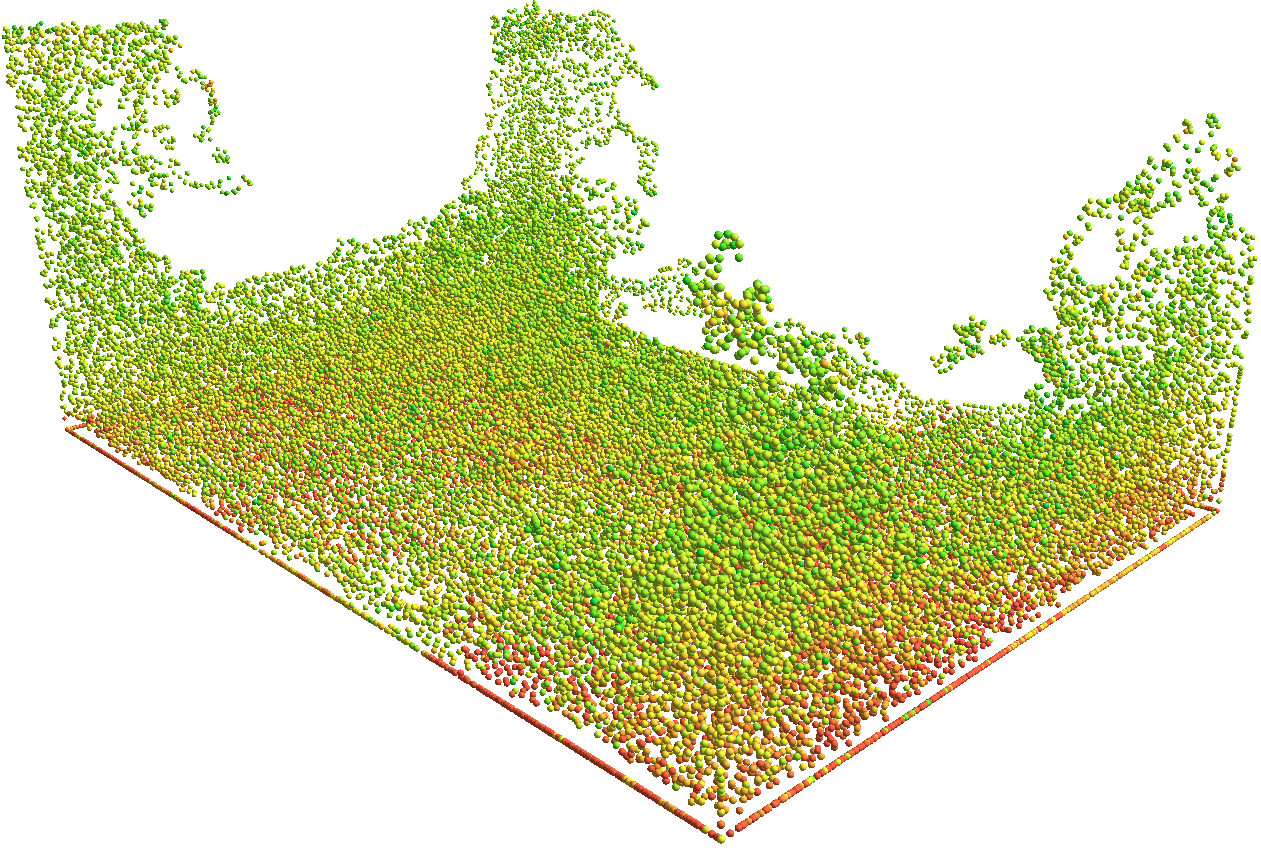
\includegraphics[width=.45\linewidth]{images/part_pressure_shader.png}}
    \caption{Visualization of the \texttt{Particle} attributes.}\label{fig:particleRender}
\end{figure}

\noindent
Finally, we visualized the particle attributes (i.e. velocity, position, and density) with three fragment subroutines that simply assign a color using a linear interpolation between two extreme colors (red and blue), as shown in Fig.\ref{fig:particleRender}. Note that this interpolation is performed in the HSV color space to have more eye-pleasing colors.


